% Created by tikzDevice version 0.12.3.1 on 2022-04-17 15:28:52
% !TEX encoding = UTF-8 Unicode
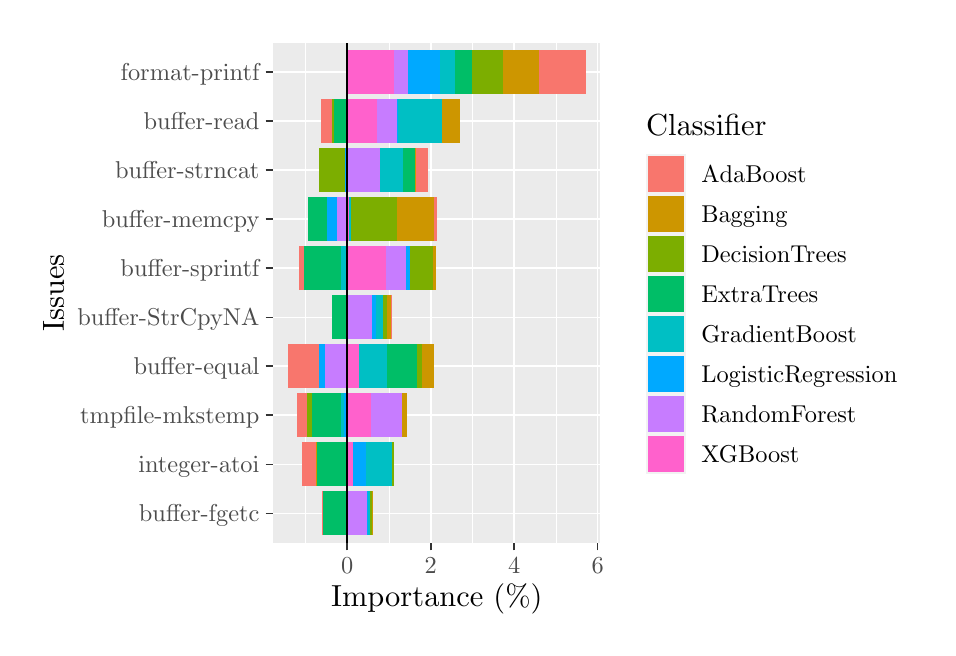
\begin{tikzpicture}[x=1pt,y=1pt]
\definecolor{fillColor}{RGB}{255,255,255}
\path[use as bounding box,fill=fillColor,fill opacity=0.00] (0,0) rectangle (325.21,216.81);
\begin{scope}
\path[clip] (  0.00,  0.00) rectangle (325.21,216.81);
\definecolor{drawColor}{RGB}{255,255,255}
\definecolor{fillColor}{RGB}{255,255,255}

\path[draw=drawColor,line width= 0.6pt,line join=round,line cap=round,fill=fillColor] (  0.00,  0.00) rectangle (325.21,216.81);
\end{scope}
\begin{scope}
\path[clip] ( 88.70, 30.69) rectangle (206.96,211.31);
\definecolor{fillColor}{gray}{0.92}

\path[fill=fillColor] ( 88.70, 30.69) rectangle (206.96,211.31);
\definecolor{drawColor}{RGB}{255,255,255}

\path[draw=drawColor,line width= 0.3pt,line join=round] (100.41, 30.69) --
	(100.41,211.31);

\path[draw=drawColor,line width= 0.3pt,line join=round] (130.57, 30.69) --
	(130.57,211.31);

\path[draw=drawColor,line width= 0.3pt,line join=round] (160.72, 30.69) --
	(160.72,211.31);

\path[draw=drawColor,line width= 0.3pt,line join=round] (190.88, 30.69) --
	(190.88,211.31);

\path[draw=drawColor,line width= 0.6pt,line join=round] ( 88.70, 41.31) --
	(206.96, 41.31);

\path[draw=drawColor,line width= 0.6pt,line join=round] ( 88.70, 59.02) --
	(206.96, 59.02);

\path[draw=drawColor,line width= 0.6pt,line join=round] ( 88.70, 76.73) --
	(206.96, 76.73);

\path[draw=drawColor,line width= 0.6pt,line join=round] ( 88.70, 94.44) --
	(206.96, 94.44);

\path[draw=drawColor,line width= 0.6pt,line join=round] ( 88.70,112.14) --
	(206.96,112.14);

\path[draw=drawColor,line width= 0.6pt,line join=round] ( 88.70,129.85) --
	(206.96,129.85);

\path[draw=drawColor,line width= 0.6pt,line join=round] ( 88.70,147.56) --
	(206.96,147.56);

\path[draw=drawColor,line width= 0.6pt,line join=round] ( 88.70,165.27) --
	(206.96,165.27);

\path[draw=drawColor,line width= 0.6pt,line join=round] ( 88.70,182.98) --
	(206.96,182.98);

\path[draw=drawColor,line width= 0.6pt,line join=round] ( 88.70,200.69) --
	(206.96,200.69);

\path[draw=drawColor,line width= 0.6pt,line join=round] (115.49, 30.69) --
	(115.49,211.31);

\path[draw=drawColor,line width= 0.6pt,line join=round] (145.65, 30.69) --
	(145.65,211.31);

\path[draw=drawColor,line width= 0.6pt,line join=round] (175.80, 30.69) --
	(175.80,211.31);

\path[draw=drawColor,line width= 0.6pt,line join=round] (205.96, 30.69) --
	(205.96,211.31);
\definecolor{fillColor}{RGB}{248,118,109}

\path[fill=fillColor] (184.85,192.72) rectangle (201.59,208.65);

\path[fill=fillColor] (105.84,175.01) rectangle (110.06,190.95);

\path[fill=fillColor] (140.07,157.30) rectangle (144.59,173.24);

\path[fill=fillColor] (147.00,139.59) rectangle (148.06,155.53);

\path[fill=fillColor] ( 98.00,121.88) rectangle ( 99.96,137.82);

\path[fill=fillColor] (131.32,104.18) rectangle (131.47,120.11);

\path[fill=fillColor] ( 94.08, 86.47) rectangle (105.24,102.40);

\path[fill=fillColor] ( 97.24, 68.76) rectangle (101.01, 84.70);

\path[fill=fillColor] ( 99.05, 51.05) rectangle (104.18, 66.99);

\path[fill=fillColor] (106.44, 33.34) rectangle (106.59, 49.28);
\definecolor{fillColor}{RGB}{205,150,0}

\path[fill=fillColor] (171.88,192.72) rectangle (184.85,208.65);

\path[fill=fillColor] (149.57,175.01) rectangle (156.35,190.95);

\path[fill=fillColor] (139.92,157.30) rectangle (140.07,173.24);

\path[fill=fillColor] (133.28,139.59) rectangle (147.00,155.53);

\path[fill=fillColor] (146.40,121.88) rectangle (147.46,137.82);

\path[fill=fillColor] (129.96,104.18) rectangle (131.32,120.11);

\path[fill=fillColor] (142.48, 86.47) rectangle (147.00,102.40);

\path[fill=fillColor] (135.39, 68.76) rectangle (137.05, 84.70);

\path[fill=fillColor] (104.18, 51.05) rectangle (104.48, 66.99);

\path[fill=fillColor] (124.54, 33.34) rectangle (124.69, 49.28);
\definecolor{fillColor}{RGB}{124,174,0}

\path[fill=fillColor] (160.57,192.72) rectangle (171.88,208.65);

\path[fill=fillColor] (110.06,175.01) rectangle (110.66,190.95);

\path[fill=fillColor] (105.09,157.30) rectangle (114.74,173.24);

\path[fill=fillColor] (117.00,139.59) rectangle (133.28,155.53);

\path[fill=fillColor] (138.11,121.88) rectangle (146.40,137.82);

\path[fill=fillColor] (128.46,104.18) rectangle (129.96,120.11);

\path[fill=fillColor] (140.52, 86.47) rectangle (142.48,102.40);

\path[fill=fillColor] (101.01, 68.76) rectangle (102.82, 84.70);

\path[fill=fillColor] (131.47, 51.05) rectangle (132.38, 66.99);

\path[fill=fillColor] (123.78, 33.34) rectangle (124.54, 49.28);
\definecolor{fillColor}{RGB}{0,190,103}

\path[fill=fillColor] (154.39,192.72) rectangle (160.57,208.65);

\path[fill=fillColor] (110.66,175.01) rectangle (115.49,190.95);

\path[fill=fillColor] (135.69,157.30) rectangle (139.92,173.24);

\path[fill=fillColor] (101.17,139.59) rectangle (108.25,155.53);

\path[fill=fillColor] ( 99.96,121.88) rectangle (113.08,137.82);

\path[fill=fillColor] (109.91,104.18) rectangle (115.49,120.11);

\path[fill=fillColor] (129.81, 86.47) rectangle (140.52,102.40);

\path[fill=fillColor] (102.82, 68.76) rectangle (113.23, 84.70);

\path[fill=fillColor] (104.48, 51.05) rectangle (115.34, 66.99);

\path[fill=fillColor] (106.59, 33.34) rectangle (115.49, 49.28);
\definecolor{fillColor}{RGB}{0,191,196}

\path[fill=fillColor] (149.11,192.72) rectangle (154.39,208.65);

\path[fill=fillColor] (133.58,175.01) rectangle (149.57,190.95);

\path[fill=fillColor] (127.40,157.30) rectangle (135.69,173.24);

\path[fill=fillColor] (116.09,139.59) rectangle (117.00,155.53);

\path[fill=fillColor] (113.08,121.88) rectangle (115.49,137.82);

\path[fill=fillColor] (125.74,104.18) rectangle (128.46,120.11);

\path[fill=fillColor] (119.71, 86.47) rectangle (129.81,102.40);

\path[fill=fillColor] (113.23, 68.76) rectangle (114.43, 84.70);

\path[fill=fillColor] (122.43, 51.05) rectangle (131.47, 66.99);

\path[fill=fillColor] (123.03, 33.34) rectangle (123.78, 49.28);
\definecolor{fillColor}{RGB}{0,169,255}

\path[fill=fillColor] (137.35,192.72) rectangle (149.11,208.65);

\path[fill=fillColor] (133.43,175.01) rectangle (133.58,190.95);

\path[fill=fillColor] (114.74,157.30) rectangle (115.49,173.24);

\path[fill=fillColor] (108.25,139.59) rectangle (111.87,155.53);

\path[fill=fillColor] (136.60,121.88) rectangle (138.11,137.82);

\path[fill=fillColor] (124.39,104.18) rectangle (125.74,120.11);

\path[fill=fillColor] (105.24, 86.47) rectangle (107.35,102.40);

\path[fill=fillColor] (114.43, 68.76) rectangle (115.49, 84.70);

\path[fill=fillColor] (117.60, 51.05) rectangle (122.43, 66.99);

\path[fill=fillColor] (122.73, 33.34) rectangle (123.03, 49.28);
\definecolor{fillColor}{RGB}{199,124,255}

\path[fill=fillColor] (132.38,192.72) rectangle (137.35,208.65);

\path[fill=fillColor] (126.20,175.01) rectangle (133.43,190.95);

\path[fill=fillColor] (115.49,157.30) rectangle (127.40,173.24);

\path[fill=fillColor] (111.87,139.59) rectangle (115.49,155.53);

\path[fill=fillColor] (129.51,121.88) rectangle (136.60,137.82);

\path[fill=fillColor] (115.49,104.18) rectangle (124.39,120.11);

\path[fill=fillColor] (107.35, 86.47) rectangle (115.49,102.40);

\path[fill=fillColor] (123.93, 68.76) rectangle (135.39, 84.70);

\path[fill=fillColor] (115.34, 51.05) rectangle (115.49, 66.99);

\path[fill=fillColor] (115.49, 33.34) rectangle (122.73, 49.28);
\definecolor{fillColor}{RGB}{255,97,204}

\path[fill=fillColor] (115.49,192.72) rectangle (132.38,208.65);

\path[fill=fillColor] (115.49,175.01) rectangle (126.20,190.95);

\path[fill=fillColor] (115.49,157.30) rectangle (115.49,173.24);

\path[fill=fillColor] (115.49,139.59) rectangle (116.09,155.53);

\path[fill=fillColor] (115.49,121.88) rectangle (129.51,137.82);

\path[fill=fillColor] (115.49,104.18) rectangle (115.49,120.11);

\path[fill=fillColor] (115.49, 86.47) rectangle (119.71,102.40);

\path[fill=fillColor] (115.49, 68.76) rectangle (123.93, 84.70);

\path[fill=fillColor] (115.49, 51.05) rectangle (117.60, 66.99);

\path[fill=fillColor] (115.49, 33.34) rectangle (115.49, 49.28);
\definecolor{drawColor}{RGB}{0,0,0}

\path[draw=drawColor,line width= 0.6pt,line join=round] (115.49, 30.69) -- (115.49,211.31);
\end{scope}
\begin{scope}
\path[clip] (  0.00,  0.00) rectangle (325.21,216.81);
\definecolor{drawColor}{gray}{0.30}

\node[text=drawColor,anchor=base east,inner sep=0pt, outer sep=0pt, scale=  0.88] at ( 83.75, 38.28) {buffer-fgetc};

\node[text=drawColor,anchor=base east,inner sep=0pt, outer sep=0pt, scale=  0.88] at ( 83.75, 55.99) {integer-atoi};

\node[text=drawColor,anchor=base east,inner sep=0pt, outer sep=0pt, scale=  0.88] at ( 83.75, 73.70) {tmpfile-mkstemp};

\node[text=drawColor,anchor=base east,inner sep=0pt, outer sep=0pt, scale=  0.88] at ( 83.75, 91.41) {buffer-equal};

\node[text=drawColor,anchor=base east,inner sep=0pt, outer sep=0pt, scale=  0.88] at ( 83.75,109.11) {buffer-StrCpyNA};

\node[text=drawColor,anchor=base east,inner sep=0pt, outer sep=0pt, scale=  0.88] at ( 83.75,126.82) {buffer-sprintf};

\node[text=drawColor,anchor=base east,inner sep=0pt, outer sep=0pt, scale=  0.88] at ( 83.75,144.53) {buffer-memcpy};

\node[text=drawColor,anchor=base east,inner sep=0pt, outer sep=0pt, scale=  0.88] at ( 83.75,162.24) {buffer-strncat};

\node[text=drawColor,anchor=base east,inner sep=0pt, outer sep=0pt, scale=  0.88] at ( 83.75,179.95) {buffer-read};

\node[text=drawColor,anchor=base east,inner sep=0pt, outer sep=0pt, scale=  0.88] at ( 83.75,197.65) {format-printf};
\end{scope}
\begin{scope}
\path[clip] (  0.00,  0.00) rectangle (325.21,216.81);
\definecolor{drawColor}{gray}{0.20}

\path[draw=drawColor,line width= 0.6pt,line join=round] ( 85.95, 41.31) --
	( 88.70, 41.31);

\path[draw=drawColor,line width= 0.6pt,line join=round] ( 85.95, 59.02) --
	( 88.70, 59.02);

\path[draw=drawColor,line width= 0.6pt,line join=round] ( 85.95, 76.73) --
	( 88.70, 76.73);

\path[draw=drawColor,line width= 0.6pt,line join=round] ( 85.95, 94.44) --
	( 88.70, 94.44);

\path[draw=drawColor,line width= 0.6pt,line join=round] ( 85.95,112.14) --
	( 88.70,112.14);

\path[draw=drawColor,line width= 0.6pt,line join=round] ( 85.95,129.85) --
	( 88.70,129.85);

\path[draw=drawColor,line width= 0.6pt,line join=round] ( 85.95,147.56) --
	( 88.70,147.56);

\path[draw=drawColor,line width= 0.6pt,line join=round] ( 85.95,165.27) --
	( 88.70,165.27);

\path[draw=drawColor,line width= 0.6pt,line join=round] ( 85.95,182.98) --
	( 88.70,182.98);

\path[draw=drawColor,line width= 0.6pt,line join=round] ( 85.95,200.69) --
	( 88.70,200.69);
\end{scope}
\begin{scope}
\path[clip] (  0.00,  0.00) rectangle (325.21,216.81);
\definecolor{drawColor}{gray}{0.20}

\path[draw=drawColor,line width= 0.6pt,line join=round] (115.49, 27.94) --
	(115.49, 30.69);

\path[draw=drawColor,line width= 0.6pt,line join=round] (145.65, 27.94) --
	(145.65, 30.69);

\path[draw=drawColor,line width= 0.6pt,line join=round] (175.80, 27.94) --
	(175.80, 30.69);

\path[draw=drawColor,line width= 0.6pt,line join=round] (205.96, 27.94) --
	(205.96, 30.69);
\end{scope}
\begin{scope}
\path[clip] (  0.00,  0.00) rectangle (325.21,216.81);
\definecolor{drawColor}{gray}{0.30}

\node[text=drawColor,anchor=base,inner sep=0pt, outer sep=0pt, scale=  0.88] at (115.49, 19.68) {0};

\node[text=drawColor,anchor=base,inner sep=0pt, outer sep=0pt, scale=  0.88] at (145.65, 19.68) {2};

\node[text=drawColor,anchor=base,inner sep=0pt, outer sep=0pt, scale=  0.88] at (175.80, 19.68) {4};

\node[text=drawColor,anchor=base,inner sep=0pt, outer sep=0pt, scale=  0.88] at (205.96, 19.68) {6};
\end{scope}
\begin{scope}
\path[clip] (  0.00,  0.00) rectangle (325.21,216.81);
\definecolor{drawColor}{RGB}{0,0,0}

\node[text=drawColor,anchor=base,inner sep=0pt, outer sep=0pt, scale=  1.10] at (147.83,  7.64) {Importance (\%)};
\end{scope}
\begin{scope}
\path[clip] (  0.00,  0.00) rectangle (325.21,216.81);
\definecolor{drawColor}{RGB}{0,0,0}

\node[text=drawColor,rotate= 90.00,anchor=base,inner sep=0pt, outer sep=0pt, scale=  1.10] at ( 13.08,121.00) {Issues};
\end{scope}
\begin{scope}
\path[clip] (  0.00,  0.00) rectangle (325.21,216.81);
\definecolor{fillColor}{RGB}{255,255,255}

\path[fill=fillColor] (217.96, 50.07) rectangle (319.71,191.92);
\end{scope}
\begin{scope}
\path[clip] (  0.00,  0.00) rectangle (325.21,216.81);
\definecolor{drawColor}{RGB}{0,0,0}

\node[text=drawColor,anchor=base west,inner sep=0pt, outer sep=0pt, scale=  1.10] at (223.46,177.78) {Classifier};
\end{scope}
\begin{scope}
\path[clip] (  0.00,  0.00) rectangle (325.21,216.81);
\definecolor{fillColor}{gray}{0.95}

\path[fill=fillColor] (223.46,156.75) rectangle (237.92,171.21);
\end{scope}
\begin{scope}
\path[clip] (  0.00,  0.00) rectangle (325.21,216.81);
\definecolor{fillColor}{RGB}{248,118,109}

\path[fill=fillColor] (224.17,157.46) rectangle (237.21,170.50);
\end{scope}
\begin{scope}
\path[clip] (  0.00,  0.00) rectangle (325.21,216.81);
\definecolor{fillColor}{gray}{0.95}

\path[fill=fillColor] (223.46,142.30) rectangle (237.92,156.75);
\end{scope}
\begin{scope}
\path[clip] (  0.00,  0.00) rectangle (325.21,216.81);
\definecolor{fillColor}{RGB}{205,150,0}

\path[fill=fillColor] (224.17,143.01) rectangle (237.21,156.04);
\end{scope}
\begin{scope}
\path[clip] (  0.00,  0.00) rectangle (325.21,216.81);
\definecolor{fillColor}{gray}{0.95}

\path[fill=fillColor] (223.46,127.84) rectangle (237.92,142.30);
\end{scope}
\begin{scope}
\path[clip] (  0.00,  0.00) rectangle (325.21,216.81);
\definecolor{fillColor}{RGB}{124,174,0}

\path[fill=fillColor] (224.17,128.56) rectangle (237.21,141.59);
\end{scope}
\begin{scope}
\path[clip] (  0.00,  0.00) rectangle (325.21,216.81);
\definecolor{fillColor}{gray}{0.95}

\path[fill=fillColor] (223.46,113.39) rectangle (237.92,127.84);
\end{scope}
\begin{scope}
\path[clip] (  0.00,  0.00) rectangle (325.21,216.81);
\definecolor{fillColor}{RGB}{0,190,103}

\path[fill=fillColor] (224.17,114.10) rectangle (237.21,127.13);
\end{scope}
\begin{scope}
\path[clip] (  0.00,  0.00) rectangle (325.21,216.81);
\definecolor{fillColor}{gray}{0.95}

\path[fill=fillColor] (223.46, 98.94) rectangle (237.92,113.39);
\end{scope}
\begin{scope}
\path[clip] (  0.00,  0.00) rectangle (325.21,216.81);
\definecolor{fillColor}{RGB}{0,191,196}

\path[fill=fillColor] (224.17, 99.65) rectangle (237.21,112.68);
\end{scope}
\begin{scope}
\path[clip] (  0.00,  0.00) rectangle (325.21,216.81);
\definecolor{fillColor}{gray}{0.95}

\path[fill=fillColor] (223.46, 84.48) rectangle (237.92, 98.94);
\end{scope}
\begin{scope}
\path[clip] (  0.00,  0.00) rectangle (325.21,216.81);
\definecolor{fillColor}{RGB}{0,169,255}

\path[fill=fillColor] (224.17, 85.19) rectangle (237.21, 98.23);
\end{scope}
\begin{scope}
\path[clip] (  0.00,  0.00) rectangle (325.21,216.81);
\definecolor{fillColor}{gray}{0.95}

\path[fill=fillColor] (223.46, 70.03) rectangle (237.92, 84.48);
\end{scope}
\begin{scope}
\path[clip] (  0.00,  0.00) rectangle (325.21,216.81);
\definecolor{fillColor}{RGB}{199,124,255}

\path[fill=fillColor] (224.17, 70.74) rectangle (237.21, 83.77);
\end{scope}
\begin{scope}
\path[clip] (  0.00,  0.00) rectangle (325.21,216.81);
\definecolor{fillColor}{gray}{0.95}

\path[fill=fillColor] (223.46, 55.57) rectangle (237.92, 70.03);
\end{scope}
\begin{scope}
\path[clip] (  0.00,  0.00) rectangle (325.21,216.81);
\definecolor{fillColor}{RGB}{255,97,204}

\path[fill=fillColor] (224.17, 56.29) rectangle (237.21, 69.32);
\end{scope}
\begin{scope}
\path[clip] (  0.00,  0.00) rectangle (325.21,216.81);
\definecolor{drawColor}{RGB}{0,0,0}

\node[text=drawColor,anchor=base west,inner sep=0pt, outer sep=0pt, scale=  0.88] at (243.42,160.95) {AdaBoost};
\end{scope}
\begin{scope}
\path[clip] (  0.00,  0.00) rectangle (325.21,216.81);
\definecolor{drawColor}{RGB}{0,0,0}

\node[text=drawColor,anchor=base west,inner sep=0pt, outer sep=0pt, scale=  0.88] at (243.42,146.50) {Bagging};
\end{scope}
\begin{scope}
\path[clip] (  0.00,  0.00) rectangle (325.21,216.81);
\definecolor{drawColor}{RGB}{0,0,0}

\node[text=drawColor,anchor=base west,inner sep=0pt, outer sep=0pt, scale=  0.88] at (243.42,132.04) {DecisionTrees};
\end{scope}
\begin{scope}
\path[clip] (  0.00,  0.00) rectangle (325.21,216.81);
\definecolor{drawColor}{RGB}{0,0,0}

\node[text=drawColor,anchor=base west,inner sep=0pt, outer sep=0pt, scale=  0.88] at (243.42,117.59) {ExtraTrees};
\end{scope}
\begin{scope}
\path[clip] (  0.00,  0.00) rectangle (325.21,216.81);
\definecolor{drawColor}{RGB}{0,0,0}

\node[text=drawColor,anchor=base west,inner sep=0pt, outer sep=0pt, scale=  0.88] at (243.42,103.13) {GradientBoost};
\end{scope}
\begin{scope}
\path[clip] (  0.00,  0.00) rectangle (325.21,216.81);
\definecolor{drawColor}{RGB}{0,0,0}

\node[text=drawColor,anchor=base west,inner sep=0pt, outer sep=0pt, scale=  0.88] at (243.42, 88.68) {LogisticRegression};
\end{scope}
\begin{scope}
\path[clip] (  0.00,  0.00) rectangle (325.21,216.81);
\definecolor{drawColor}{RGB}{0,0,0}

\node[text=drawColor,anchor=base west,inner sep=0pt, outer sep=0pt, scale=  0.88] at (243.42, 74.23) {RandomForest};
\end{scope}
\begin{scope}
\path[clip] (  0.00,  0.00) rectangle (325.21,216.81);
\definecolor{drawColor}{RGB}{0,0,0}

\node[text=drawColor,anchor=base west,inner sep=0pt, outer sep=0pt, scale=  0.88] at (243.42, 59.77) {XGBoost};
\end{scope}
\end{tikzpicture}
